%%%% Header %%%%%%%%%%%%%%%%%%%%%%%%%%%%%%%%%%%%%%%%%%%%%%%%%%%%%%%%%%%%%%%%%%%

\documentclass{beamer}

\usepackage{jobeam}

% bibliography file
\bibliography{/home/jon/lucile/share/jowncloud/sci/refs/refs.bib}

%%%% Meta Data %%%%%%%%%%%%%%%%%%%%%%%%%%%%%%%%%%%%%%%%%%%%%%%%%%%%%%%%%%%%%%%%

\title{Visualizing Composite Data on the Lexis Surface}
\subtitle{What share of a population features\\attribute $i$ at period $t$ and age $x$?}
\author{Jonas Schöley\\\url{schoeley@demogr.mpg.de}}
%\institute{\includegraphics[width = 3cm]{../fig/talk/EDSDLogo.pdf}}
\subject{Visualizing composite data on the Lexis surface}
\keywords{data visualization, compositional data, Lexis surface, causes of death}

\begin{document}

%%%% Titlepage %%%%%%%%%%%%%%%%%%%%%%%%%%%%%%%%%%%%%%%%%%%%%%%%%%%%%%%%%%%%%%%%

{
  \usebackgroundtemplate{\includegraphics[width=\paperwidth]{../fig/talk/background.png}}%
  \begin{frame}[plain]
    \titlepage
  \end{frame}
}

%%%% Slides %%%%%%%%%%%%%%%%%%%%%%%%%%%%%%%%%%%%%%%%%%%%%%%%%%%%%%%%%%%%%%%%%%%

\section{Predefined Visual Spaces} %%%%%%%%%%%%%%%%%%%%%%%%%%%%%%%%%%%%%%%%%%%%

\begin{frame}{pause}
\frametitle{\insertsection}

\begin{columns}[c]

\column{0.73\textwidth}
\begin{figure}[!htb]
\centering
\begin{subfigure}[c]{\textwidth}
\includegraphics[width = \textwidth]{../fig/talk/spatial_map_empty.pdf}
\end{subfigure}\\
\begin{subfigure}[c]{\textwidth}
\includegraphics[width = \textwidth]{../fig/talk/temporal_map_empty.pdf}
\end{subfigure}
\end{figure}

\column{0.27\textwidth}
\footnotesize\textbf{A spatial map}.

\vspace{2.5cm}

\footnotesize\textbf{A temporal map}.

\end{columns}

\end{frame}

%%%%%%%%%%%%%%%%%%%%%%%%%%%%%%%%%%%%%%%%%%%%%%%%%%%%%%%%%%%%%%%%%%%%%%%%%%%%%%%

\begin{frame}{pause}
\frametitle{\insertsection}

\begin{columns}[c]

\column{0.73\textwidth}
\begin{figure}[!htb]
\centering
\begin{subfigure}[c]{\textwidth}
\includegraphics[width = \textwidth]{../fig/talk/spatial_map.pdf}
\end{subfigure}\\
\begin{subfigure}[c]{\textwidth}
\includegraphics[width = \textwidth]{../fig/talk/temporal_map.pdf}
\end{subfigure}
\end{figure}

\column{0.27\textwidth}
\footnotesize\textbf{A spatial map}\\ The surface of Mars with elevation encoded by colour. \scriptsize\emph{NASA 2000}.

\vspace{2.5cm}

\footnotesize\textbf{A temporal map}\\ Fertility rates in Scotland since 1945 with rate encoded by colour. \scriptsize\emph{Modified from \cite{Riffe2011}.}

\end{columns}

\end{frame}

\section{Plotting Data: Magnitudes vs.~Compositions} %%%%%%%%%%%%%%%%%%%%%%%%%%

\begin{frame}
\frametitle{\insertsection}

$$
\begin{matrix*}[c]
\mbox{\Large$\mathit{Easy}$} & & \mbox{\Large$\mathfrak{Hard}$} \\\midrule
187 \dfrac {\text{Deaths}} {10\,000~\text{Persons}} &
\Longleftarrow &
\begin{pmatrix*}[l]
93 & \text{Neoplasm} \\
40 & \text{Cardiovascular} \\
23 & \text{Respiratory} \\
12 & \text{Accident} \\
19 & \text{Other}
\end{pmatrix*} \\
\text{Single~value} & \text{composed~of} & \text{n-dimensional~vector} \\
& & & \\
& & \Downarrow \text{expressed~as} \\
& & & \\
& & \begin{pmatrix*}[l]
0.50 & \text{Neoplasm} \\
0.21 & \text{Cardiovascular} \\
0.12 & \text{Respiratory} \\
0.06 & \text{Accident} \\
0.11 & \text{Other}
\end{pmatrix*} \\
& & \text{n-dimensional simplex}
\end{matrix*}
$$

\end{frame}

\section{Binary Compositions on a Surface} %%%%%%%%%%%%%%%%%%%%%%%%%%%%%%%%%%%%

\begin{frame}
\frametitle{\insertsection}

\begin{figure}[htb!]
\includegraphics[width = \textwidth]{../fig/talk/binary.png} \\
\small \textbf{Divergent colour scale}\\ US presidential election 2012.\\Proportion of people voting for Democrats vs. Republicans.\\\scriptsize\emph{\cite{GuardianGraphics2012}.}
\end{figure}

\end{frame}

\section{Ternary Compositions on a Surface} %%%%%%%%%%%%%%%%%%%%%%%%%%%%%%%%%%%

\begin{frame}
\frametitle{\insertsection}

\begin{columns}[c]

\column{0.57\textwidth}
\begin{figure}[htb!]
\includegraphics[width = 0.97\textwidth]{../fig/talk/tern_balance_no_lgnd.pdf}
\end{figure}

\column{0.37\textwidth}
\small \textbf{Ternary-balance-scheme}\\ Proportion of people dying from a given cause by time and age. \scriptsize\emph{France, total population.}

\begin{figure}[htb!]
\includegraphics[width = \textwidth]{../fig/talk/tern_balance_lgnd.pdf}
\end{figure}

\end{columns}

\end{frame}

\section{N-dimensional compositions on a surface} %%%%%%%%%%%%%%%%%%%%%%%%%%%%%

\subsection{Qualitative Sequential Scheme}

\begin{frame}
\frametitle{\insertsection}

\begin{columns}[c]

\column{0.7\textwidth}
\begin{figure}[htb!]
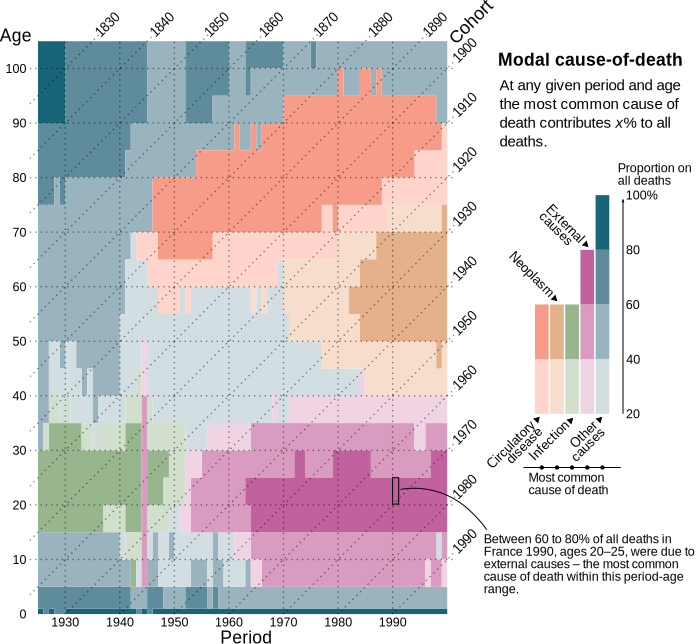
\includegraphics[width = 0.97\textwidth]{../fig/talk/qual_seq.pdf}
\end{figure}

\column{0.3\textwidth}
\footnotesize \textbf{Qualitative sequential scheme}\\ Proportion of people dying from the most prominent cause in a given time and age. \scriptsize\emph{France, total population.}

\end{columns}

\end{frame}

\section{Interlude: Brewers Typology of Colour Schemes} %%%%%%%%%%%%%%%%%%%%%%%

\begin{frame}
\frametitle{\insertsection}

\begin{columns}[c]

\column{0.75\textwidth}
\begin{figure}[htb!]
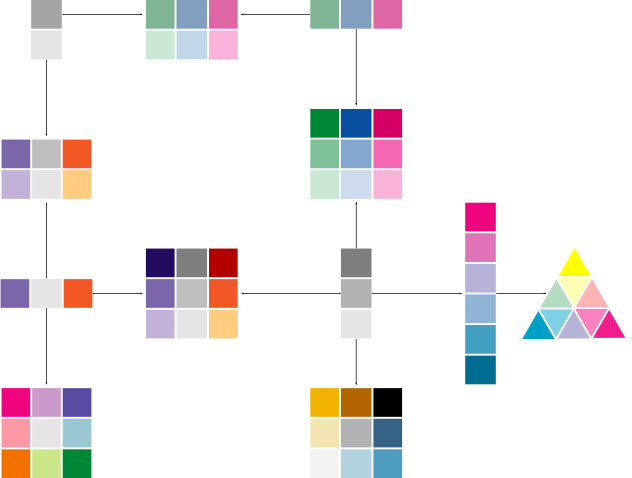
\includegraphics[width = \textwidth]{../fig/talk/brewer_typology.pdf}\\
\end{figure}

\column{0.25\textwidth}
\footnotesize\textbf{Colour scheme typology}\\ Basic colour schemes and combinations of them. \scriptsize\emph{Redrawn from \textcite{Brewer1994}.}

\end{columns}

\end{frame}

\section{Cont'd: N-dimensional Compositions on a Surface} %%%%%%%%%%%%%%%%%%%%%

\subsection{Age-wise Area Chart}

\begin{frame}
\frametitle{\insertsection}

\begin{columns}[c]

\column{0.7\textwidth}
\begin{figure}[htb!]
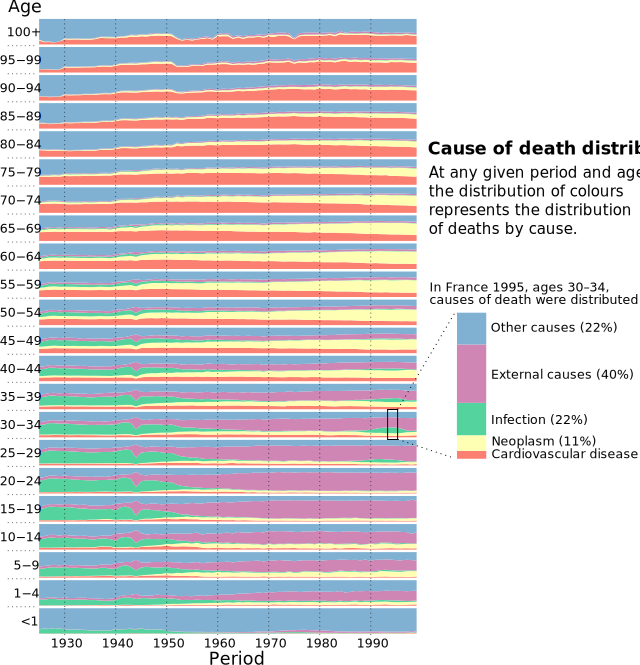
\includegraphics[width = 0.93\textwidth]{../fig/talk/agewise_area.pdf}
\end{figure}

\column{0.3\textwidth}
\small \textbf{Age-wise-area-chart}\\ Proportion of people dying from a given cause by time and age. \scriptsize\emph{France, total population.}

\end{columns}

\end{frame}

%

\subsection{Small Multiples}

\begin{frame}
\frametitle{\insertsection}

\begin{figure}[htb!]
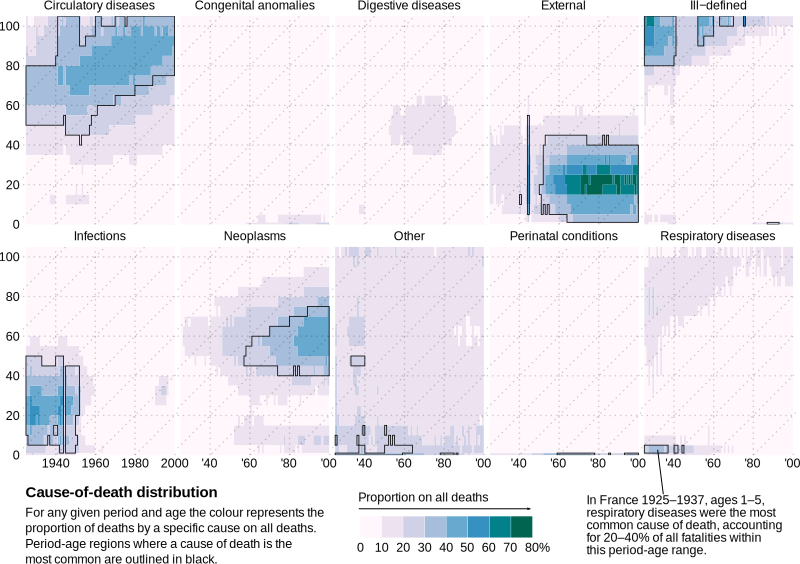
\includegraphics[width = \textwidth]{../fig/talk/small_multiples.pdf}\\
\scriptsize \textbf{Small-multiples}\\ Proportion of people dying from a given cause by time and age. \tiny\emph{France, total population.}
\end{figure}

\end{frame}

\section{References} %%%%%%%%%%%%%%%%%%%%%%%%%%%%%%%%%%%%%%%%%%%%%%%%%%%%%%%%%%

\begin{frame}
\frametitle{\insertsection}

\begin{centering}

\Large\fullcite{Schoeley2015}

\smallskip

\Large\texttt{https://github.com/jschoeley/viscomplexis}

\end{centering}

\end{frame}

%%%%%%%%%%%%%%%%%%%%%%%%%%%%%%%%%%%%%%%%%%%%%%%%%%%%%%%%%%%%%%%%%%%%%%%%%%%%%%%

\begin{frame}
\frametitle{\insertsection}

\nocite{MOLAST2000}

\printbibliography

\end{frame}

\end{document}